\documentclass[
%draft%     uncomment to activate draft mode (see preamble/proofs)
]{article}   

% preamble -- do not rearrange order of \includes
%\include{classoptions}
%\include{pagesize}
%\include{packages}
%\include{encoding}         
%\include{fonts}
%\include{ToC}
%\include{contributor}
%\include{copyright}
%\include{bibtex}
%\include{environments}
%\include{sectionoptions}
%\include{headerfooter}
%\include{footnoteformat}
%\include{codesnipets}
%\include{proofs}
\usepackage{algorithm}% http://ctan.org/pkg/algorithms
\usepackage{algpseudocode}% http://ctan.org/pkg/algorithmicx
\usepackage[style=numeric,sorting=none]{biblatex}
\addbibresource{main.bib} %Import the bibliography file
\usepackage{tikz}
\usepackage{graphicx}
\usepackage[export]{adjustbox}
\usepackage{caption}
\usepackage{amssymb}
\usepackage{float}
\usepackage{subfig}
\usepackage{placeins}
\usepackage{listings}
\lstset{
  basicstyle=\ttfamily,
  mathescape
}
%\usepackage{minted}
\usetikzlibrary{shapes}
\usetikzlibrary {positioning}
\usetikzlibrary{chains}
\usetikzlibrary{fit}
\usetikzlibrary{chains,shadows.blur}
\usepackage{geometry}
\usepackage{array}
\usepackage{hyperref}
\usepackage{indentfirst}
\hypersetup{
    colorlinks=true,
    linkcolor=magenta,
    filecolor=cyan,      
    urlcolor=blue,
}
\graphicspath{ {./images/} }


\usepackage{listings}
\usepackage{xcolor}

\definecolor{codegreen}{rgb}{0,0.6,0}
\definecolor{codegray}{rgb}{0.5,0.5,0.5}
\definecolor{codepurple}{rgb}{0.58,0,0.82}
\definecolor{backcolour}{rgb}{0.95,0.95,0.92}

\lstdefinestyle{mystyle}{
    % backgroundcolor=\color{backcolour},   
    commentstyle=\color{codegreen},
    keywordstyle=\color{magenta},
    numberstyle=\tiny\color{codegray},
    stringstyle=\color{codepurple},
    basicstyle=\ttfamily\footnotesize,
    breakatwhitespace=false,         
    breaklines=true,                 
    captionpos=b,                    
    keepspaces=true,                 
    numbers=left,                    
    numbersep=5pt,                  
    showspaces=false,                
    showstringspaces=false,
    showtabs=false,                  
    tabsize=2
}

\lstset{style=mystyle}


% define issue details
\title{Compiler Optimization Notes}
\newcommand\thejournalsubtitle{Notes for the Compiler Optimization Techniques}
\newcommand\thevolume{}
\newcommand\theseason{May}
\newcommand\theyear{2022}
\newcommand\theissue{\thejournal \ \thevolume \ (\theyear)} 

\newcommand\generaleditor{}
\newcommand\associateeditor{}
\sloppy
\newcommand\thewebsite{https://github.com/liusy58/CompilerNotes}

\begin{document}
\sloppy                         % preferences more space between words over overrunning margins
\lefthyphenmin=3                % suppresses hyphenation after only 1 or 2 characters
                                % NB: You will need to repeat \lefthyphenmin in the text if you use \selectlanguage
%\include{editorialboard}
%\include{titlepage}
%\include{colofon}
\pagenumbering{roman}           
%\tableofcontents  
\thispagestyle{empty}

\maketitle


% \include{essays/preface}
\pagenumbering{arabic}

\section{Local Optimizations}

Local Optimizations never goes away because this is always a piece of what happens even when we 
talk about even more sophiscated types of optimizations.

First we will talk about how to represent the code within a function or procedure, that's using 
something called a flow graph which is made of basic blocks.  Next we will contrast two different 
abstractions for doing local optimizations.




\subsection{Basic Blocks/Flow graphs} 


\subsubsection{Basic Blocks}

A basic block is a sequence of instructions(3-address statements). There are some requirements for basic 
block:

\begin{itemize}
    \item \textbf{Only the first instruction can be reached from outside the blcok.} The reason why this property 
    is useful is that within a basic block, we just march instruction by instruction through the block, 
    this simplies things at least within a basic block.
    \item \textbf{All the statements are executed consecutively if the first one is.}
    \item \textbf{The basic block must be maximal.} i.e., they cannot be made larger without violating conditions. 
\end{itemize}


\subsubsection{Flow graphs}
Flow graph is a graph representation of the procedure. In flow graph, basic blocks are the nodes, and the edge for \(  B_i 
\rightarrow B_j \) stands for a path from node \( B_i \) to node \( B_j \). So how will \(  B_i  \rightarrow B_j \) happen? 
There are two possibilities:

\begin{itemize}
    \item Either first instruction of \(B_j\) is the target of a goto at end of \(B_i\).
    \item \(B_j\) physically follows \(B_i\) which doesn't end in an unconditional goto.
\end{itemize}




% \begin{center}

% \begin{tikzpicture}[auto,
%     node distance = 12mm,
%     start chain = going below,
%     box/.style = {draw,rounded corners,blur shadow,fill=white,
%           on chain,align=center}]
%    \node[box] (b1)    {$x_1\leftarrow0$\\ $y_1\leftarrow0$};      
%    \node[box] (b2)    {$x_2\leftarrow\phi(x_1,x_3)$\\
%    $y_2\leftarrow\phi(y_1,y_3)$\\
%    $(x_2<10)$?};      
%    \node[box] (b3)    {$y_3\leftarrow y_2+x_2$\\ $x_3\leftarrow x_2+1$};  
%    \node[box] (b4)    {print($y_2$)};     
%    \begin{scope}[rounded corners,-latex]
%     \path (b2.-40) edge[bend left=50] (b4.40)
%     (b1) edge (b2) (b2) edge (b3);
%     \draw (b3.230) -- ++(0,-0.3) -| ([xshift=-5mm]b2.west) |-
%     ([yshift=3mm]b2.130) -- (b2.130);
%    \end{scope}
%   \end{tikzpicture}

% \end{center}




\subsubsection{Partitioning into Basic Blocks}

\begin{itemize}
\item Identify the leader of each basic block 
    \begin{itemize}
        \item First instruction
        \item Any target of a jump
        \item Any instruction immediately following a jump
    \end{itemize}

\item Basic block starts at leader and ends at instruction immediately before a leader(or the last instruction).    
\end{itemize}

An example of flow graph is shown below:

\begin{figure}[h]
    \centering
    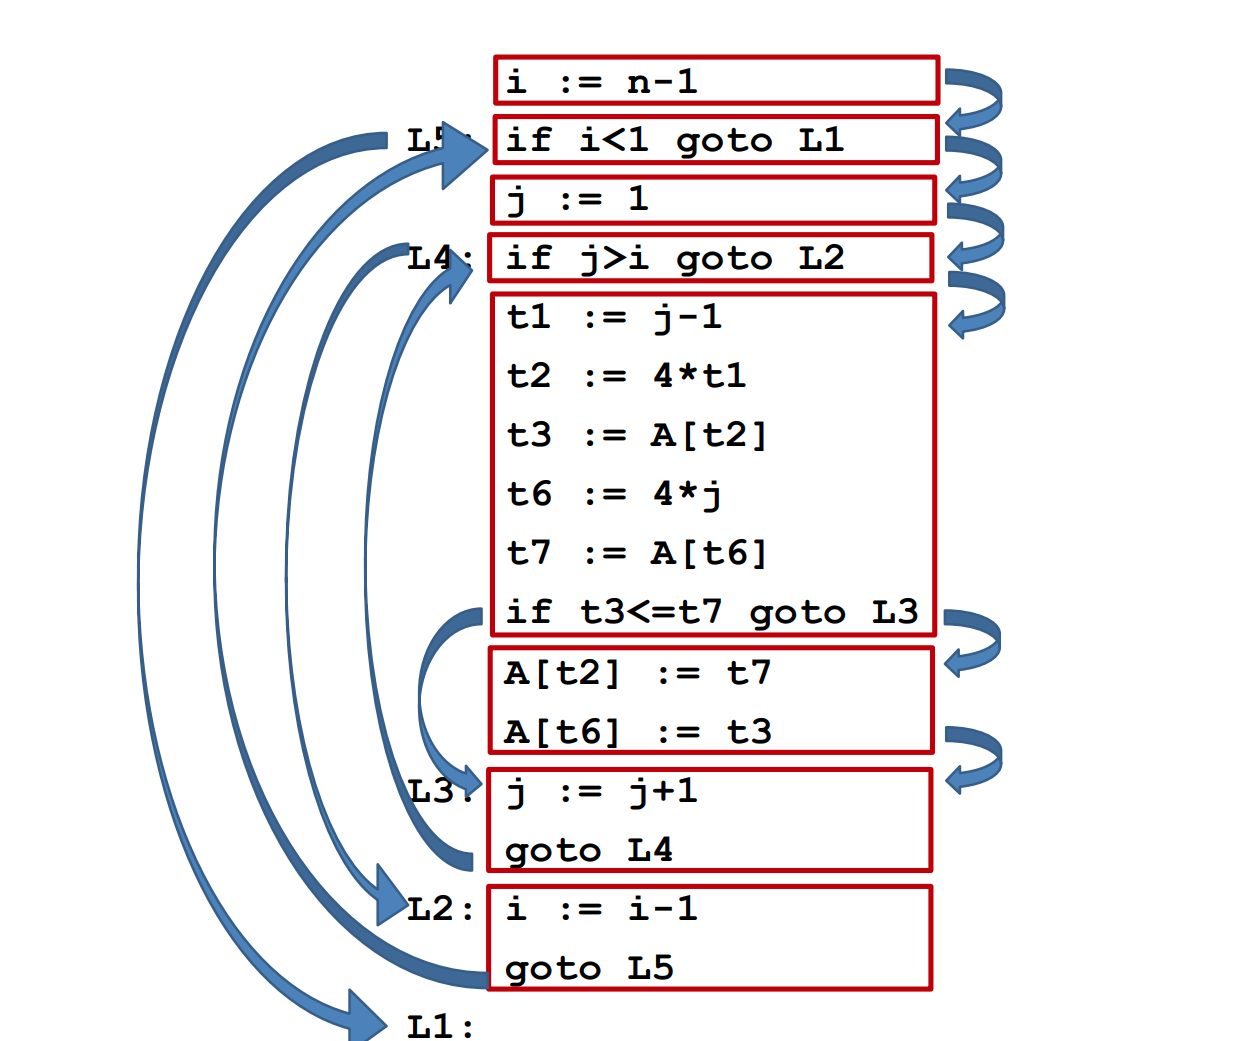
\includegraphics[width=0.5\textwidth]{flowgraph.png}
    \caption{Example of a flow graph}
\end{figure}

\subsubsection{Reachability of Basic Blocks}

There is one thing interesting need to mention here. So the source code is below:

\begin{lstlisting}[language=C, caption=An example]
if x { 
    ...
    return;
} else {
    ...
}


\end{lstlisting}


The corresponding flow graph is shown in \ref{fig:fgex}:

\begin{figure}[h]
    \centering
    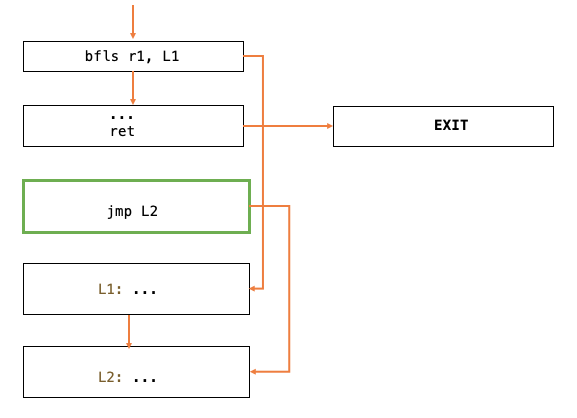
\includegraphics[width=0.5\textwidth]{fgex.png}
    \caption{Example of a flow graph}
    \label{fig:fgex}
\end{figure}


We can see that the box in green is unreachable from the entry. So why is that interesting? Typically, after compiers 
construct the control flow graph, they will go through and remove any unreachable nodes. Just do depth first traversal of the graph
from the entry node and mark all those visited nodes. So unmarked nodes will be deleted. This will help the compiler get a better optimization
result.


So why do these unreachable nodes appear? The anwser is it is not the job of the front-end of the compiler to clean up the unreachable nodes. 



\subsection{Local optimizations}

Local optimizations are those occur \textbf{within the basic blocks}. 


\subsubsection{common subexpression elimination}

There're some types of local optimizations. 
One is called \textbf{common subexpression elimination}. Subexpressions are some arithmetic expressions that occur on the
 right hand of the instructions. Common subexpressions are subexpression that occur many times where the operands have not 
 changed.
 
\begin{lstlisting}[language=C, caption=Subexpression example,label=lst:subexp]
a = b + c;
d = b + c;
\end{lstlisting}

In the example \ref{lst:subexp}, \texttt{b + c} is so called coomon subexpression, we could replace the instruction containing 
common subexpression with an assign expression. 


\begin{lstlisting}[language=C, caption=code snippet applied common subexpression elimination to \ref{lst:subexp},label=lst:transsubexpr]
    a = b + c;
    d = a
\end{lstlisting}

You may wonder why this kind of redundancy can occure in code? Are we programmers stupid to do so? In fact, 
the redundancy most comes from the stage when compilers  turn your source code. For example, when you use arrays,
you need to do some arithmetic to generate the address of the array element you are accessing. So every time you referece the same
array element, compiler will calculate the same address again. Similarly, if you access offsets within fields. Last example is 
access to parameters in the stack. 


\subsection{Abtraction 1:DAG}

DAG is the acronym for Directed Acyclic Graph. The Directed Acyclic Graph (DAG) is used to represent the 
structure of basic blocks, to visualize the flow of values between basic blocks, and to provide 
optimization techniques in the basic block. DAG is an efficient method for identifying common 
sub-expressions.\footnote{copied from \url{https://wildpartyofficial.com/what-is-dag-in-compiler-construction}}



The parse tree and DAG of the expression \(a + a*(b+c) + (b+c) *d \) is shown in \ref{fig:DAG}.


\begin{figure}[h]
    \centering
    \includegraphics[width=0.5\textwidth]{DAG.png}
    \caption{Example of a DAG}
    \label{fig:DAG}
\end{figure}



In DAG, some of the computation are reused. So we can generate optimizaed code based on DAG.

The optmized code for the DAG\ref{fig:DAG} is: 

\begin{lstlisting}[language=C, caption=code ,label=lst:dag]
    t1 = b - c;
    t2 = a * t1;
    t3 = a + t2;
    t4 = t1 * d;
    t5 = t3 + t4;
\end{lstlisting}


\subsubsection{How well do DAGs hold up across statements?}

We have seen that DAGs can be useful in a long arithmetic expression. So how well do DAGs
perform in sequence of instructions?

\begin{lstlisting}[language=C, caption=code ,label=lst:dagexpr2]
    a = b + c;
    b = a - d;
    c = b + c;
    d = a - d;
\end{lstlisting}


The corresponding DAG is shown in \ref{fig:DAG2}.
\begin{figure}[h]
    \centering
    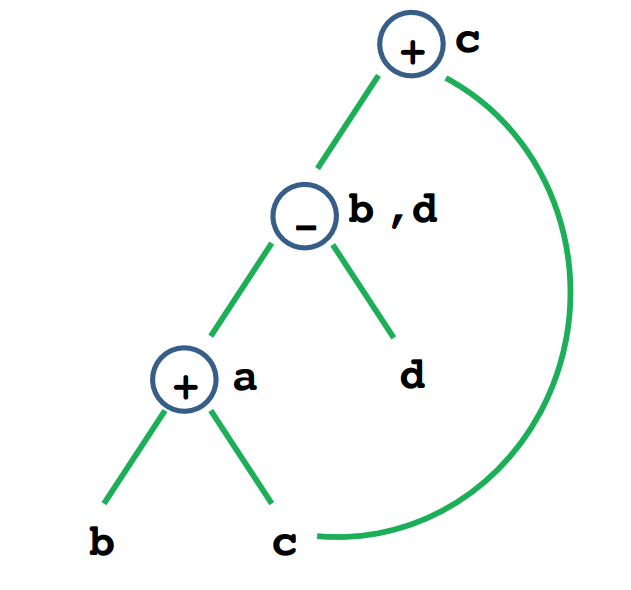
\includegraphics[width=0.5\textwidth]{dag2.png}
    \caption{Example of a DAG}
    \label{fig:DAG2}
\end{figure}

Based on the DAG\ref{fig:DAG2}, one optimizaed code is \ref{lst:dagexprop2}


\begin{lstlisting}[language=C, caption=code ,label=lst:dagexprop2]
a = b+c;
d = a-d;
c = d+c;
\end{lstlisting}

\ref{lst:dagexprop2} is not correct. B need to be overwritten but not yet. So if using DAGs, you need to be 
very careful. 

DAGs make sense if you just have one long expression, but once you have sequence of instructions overwriting variables
, DAGs are less appealing because this abstraction doesn't really include the concept of time.




\subsection{Abtraction 2:Value numbering} 

We have seen drawbacks of DAGs. One way to fix the problem is to attach variable name to latest value. Value numbering is 
such abstraction.

The idea behind value numbering is there is a mapping between variables(static) to values(dynamic). So common subexpression means same 
value number.

\subsubsection{Algorithm}


\begin{lstlisting}[language=python, caption=code ,label=lst:vna]
Data structure:
    VALUES = Table of
        expression /* [OP, valnum1, valnum2] */
        var /* name of variable currently holding expr */
For each instruction (dst = src1 OP src2) in execution order
    valnum1=var2value(src1); valnum2=var2value(src2)

    IF [OP, valnum1, valnum2] is in VALUES
        v = the index of expression
        Replace instruction with: dst = VALUES[v].var
    ELSE
        Add
            expression = [OP, valnum1, valnum2]
            var = tv
        to VALUES
        v = index of new entry; tv is new temporary for v
        Replace instruction with: tv = VALUES[valnum1].var OP VALUES[valnum2].var
                                dst = tv
    set_var2value (dst, v)  
\end{lstlisting}


\subsubsection{example}







\section{Introduction to Data Flow Analysis}

\subsection{Motivation for Dataflow Analysis}

Some optimizations\footnote{based on \url{https://pages.cs.wisc.edu/~horwitz/CS704-NOTES/2.DATAFLOW.html}} , however, require more "global" information. 
For example, consider the code \ref{lst:expr1}

\begin{lstlisting}[language=C,frame=single, caption=An ,label = lst:expr1]
    a = 1;
    b = 2;
    c = 3;
    if (...) x = a + 5;
    else x = b + 4;
    c = x + 1;
\end{lstlisting}


In this example, the initial assignment to \textit{c} (at line 3) is useless, and the expression 
\textit{x + 1} can be simplified to 7, but it is less obvious how a compiler can discover these facts 
since they cannot be discovered by looking only at one or two consecutive statements. 
A more global analysis is needed so that the compiler knows at each point in the program:
\begin{itemize}
\item    which variables are guaranteed to have constant values, and
\item    which variables will be used before being redefined.
\end{itemize}

To discover these kinds of properties, we use dataflow analysis. 



\subsubsection{What is Data Flow Analysis?}

Local Optimizations only consider optimizations within a node in CFG. 
Data flow analysis will take edges into account, which means composing 
effects of basic blocks to derive information at basic block boundaries.
Data-flow analysis is a technique for gathering information about the possible 
set of values calculated at various points in a computer program. A program's 
control-flow graph (CFG) is used to determine those parts of a program to which 
a particular value assigned to a variable might propagate. The information gathered 
is often used by compilers when optimizing a program. 


Typically, we will do local optimization for the first step to know what happens in a 
basic block, step 2 is to do data flow analysis. In he third step, we will go back and 
revisit the individual instructions inside of the blocks.


Data flow analysis is \textbf{flow-sensitive}, which means we take into account
 the effect of control flow. It is also a \textbf{intraprocedural analysis} which means
 the analysis is within a procedure. Data-flow analysis computes its solutions over the paths in
 a control-flow graph. The well-known, meet-over-all-paths
 formulation produces safe, precise solutions for general dataflow problems. All paths-whether feasible or infeasible,
 heavily or rarely executed-contribute equally to a solution. 

Here are some examples of intraprocedural optimizations:

\begin{itemize}
\item \textbf{constant propagation}. Constant propagation is a well-known global flow analysis 
problem. The goal of constant propagation is to discover values that are constant on all possible 
executions of a program and to propagate these constant values as far forward through the program 
as possible. Expressions whose operands are all constants can be evaluated at compile time and the 
results propagated further.

\item \textbf{common subexpression elimination}

\item \textbf{dead code elimination}. Actually, source code written by programmers doesn't contain
 a lot of dead code, dead code happens to occur partly because of how the front end translates code into 
 the IR. Doing optimizations will also turn code into dead.

\end{itemize}

% \subsection{Static    Program    vs.    Dynamic    Execution }

% Static program 




\subsubsection{Static Program vs. Dynamic Execution}


Program is statically infinite, but there can be infinite many dynamic execution paths. On one hand, analysis
 need to be precise, so we will take into account as much dynamic execution as possible. On the other hand, analysis
 need to do the analysis quickly. For a compromise, the analysis result is \textbf{conservative} and what it does id for each 
 point in the program, combines information of all the instances of the same program point.





\subsubsection{Data Flow Analysis Schema}
Before thinking about how to define a dataflow problem, note that there are two kinds of problems:
\begin{itemize}
    \item Forward problems (like constant propagation) where the information at a node n summarizes what can happen on paths from "enter" to n. So if we care about what happened in the past, it's a forward problem.
    \item Backward problems (like live-variable analysis), where the information at a node n summarizes what can happen on paths from n to "exit". So if we care about what will happen in the future, it's a backward problem.
\end{itemize}    

In what follows, we will assume that we're thinking about a forward problem unless otherwise specified.
 
Another way that many common dataflow problems can be categorized is as may problems or must problems. 
The solution to a "may" problem provides information about what may be true at each program point (e.g., 
for live-variables analysis, a variable is considered live after node n if its value may be used before 
being overwritten, while for constant propagation, the pair (x, v) holds before node n if x must have the value v at that point).

Now let's think about how to define a dataflow problem so that it's clear what the (best) solution should be. 
When we do dataflow analysis "by hand", we look at the CFG and think about:

\begin{itemize}
    \item What information holds at the start of the program.
    \item When a node n has more than one incoming edge in the CFG, how to combine the incoming 
    information (i.e., given the information that holds after each predecessor of n, how to 
    combine that information to determine what holds before n).
    \item How the execution of each node changes the information.
\end{itemize}    

This intuition leads to the following definition. An instance of a dataflow problem includes:
\begin{itemize}
    \item a \(CFG\),
    \item a domain \(D\) of "dataflow facts",
    \item a dataflow fact "init" (the information true at the start of the program for forward problems, 
    or at the end of the program for backward problems),
    \item an operator \(\wedge\) (used to combine incoming information from multiple predecessors),
    \item for each CFG node n, a dataflow function \(f_n\) :\( D \rightarrow D\) (that defines the effect of 
    executing n).
\end{itemize} 

For constant propagation, an individual dataflow fact is a set of pairs of the form (var, val),
 so the domain of dataflow facts is the set of all such sets of pairs (the power set). 
 For live-variable analysis, it is the power set of the set of variables in the program.

For both constant propagation and live-variable analysis, the "init" fact is the empty set 
(no variable starts with a constant value, and no variables are live at the end of the program).



For constant propagation, the combining operation \(\wedge\) is set intersection. 
This is because if a node n has two predecessors, p1 and p2, then variable x has value v before 
node n iff it has value v after both p1 and p2. For live-variable analysis, 
\(\wedge\) is set union: if a node n has two successors, s1 and s2, then the value of x after n may be 
used before being overwritten iff that holds either before s1 or before s2. In general, 
for "may" dataflow problems, \(\wedge\) will be some union-like operator, while it will be an intersection-like 
operator for "must" problems.

For constant propagation, the dataflow function associated with a CFG node that does not assign 
to any variable (e.g., a predicate) is the identity function. For a node n that assigns to 
a variable x, there are two possibilities:

\begin{itemize}
\item 1. The right-hand side has a variable that is not constant. In this case, the function 
result is the same as its input except that if variable x was constant the before n, 
it is not constant after n.
\item 2. All right-hand-side variables have constant values. In this case, the right-hand side of 
the assignment is evaluated producing consant-value c, and the dataflow-function result is the 
same as its input except that it includes the pair (x, c) for variable x (and excludes the pair 
for x, if any, that was in the input).
\end{itemize}


For live-variable analysis, the dataflow function for each node n has the form: 
\(f_n(S) = Gen_n \cup (S - KILL_n)\), where \(KILL_n\) is the set of variables defined at node n, 
and \(GEN_n\) is the set of variables used at node n. In other words, for a node that does not 
assign to any variable, the variables that are live before n are those that are live after 
n plus those that are used at n; for a node that assigns to variable x, the variables that are 
live before n are those that are live after n except x, plus those that are used at n 
(including x if it is used at n as well as being defined there).

An equivalent way of formulating the dataflow functions for live-variable analysis is: 
\(f_n(S) = (S \cap NOT-KILL_n) \cup GEN_n\), where \(NOT-KILL_n\) is the set of variables not defined
 at node n. The advantage of this formulation is that it permits the dataflow facts to be 
 represented using bit vectors, and the dataflow functions to be implemented using simple 
 bit-vector operations (and or).

It turns out that a number of interesting dataflow problems have dataflow functions of this 
same form, where \(GEN_n\) and \(KILL_n\) are sets whose definition depends only on n, and the combining 
operator \(\wedge\) is either union or intersection. These problems are called GEN/KILL problems, 
or bit-vector problems.




\subsection{Reaching Definitions}

The Reaching Definitions Problem is a data-flow problem used to answer the
following questions: Which definitions of a variable \textit{X} reach a given use of \textit{X} in
an expression? Is \textit{X} used anywhere before it is defined? A definition\textit{d} reaches a point \textit{p} if there exists path 
from the point immediately following \textit{d} to \textit{p} such that \textit{d} is not killed(overwritten) along that path.



\subsubsection{Iterative   Algorithm}

Here is the iterative  algorithm.



\begin{algorithm}
    \caption{Reaching Defintions:Iterative Algorithm}\label{alg:reachingdefiterative}
    \hspace*{\algorithmicindent} \textbf{Input: control flow graph CFG = (N, E, Entry, Exit) } \\
   
    
    \begin{algorithmic}
   
    \State out[Entry] = $\emptyset$ \algorithmiccomment{Boundary condition}

    \For{\texttt{each basic block B other than Entry}}
        \State \texttt{out[B] = $\emptyset$} \algorithmiccomment{Initialization for iterative algorithm }
    \EndFor
    \While{Changes to any out[] occur}
        \For{\texttt{each basic block B other than Entry}}
        \State \texttt{$in[B] =  \cup (out[p])$, for all predecessors p of B}
        \State \texttt{$out[B] = f_B(in[B])$} \algorithmiccomment{$out[B]=gen[B]\cup (in[B]-kill[B]) $ }
        \EndFor

    \EndWhile
    \end{algorithmic}
\end{algorithm}




\subsubsection{ Worklist   Algorithm}

\begin{algorithm}
    \caption{Reaching Defintions:Worklist Algorithm}\label{alg:reachingdefiterative}
    \hspace*{\algorithmicindent} \textbf{Input: control flow graph CFG = (N, E, Entry, Exit) } \\
   
    
    \begin{algorithmic}
   
    \State out[Entry] = $\emptyset$ \algorithmiccomment{Boundary condition}
    \State \textcolor{blue}{ChangedNodes = N}   
    \For{\texttt{each basic block B other than Entry}}
        \State \texttt{out[B] = $\emptyset$} \algorithmiccomment{Initialization for iterative algorithm }
    \EndFor
    \While{ChangedNodes $\neq \emptyset$}
        \State \textcolor{blue}{Remove i from ChangedNodes}
        \State $in[B] =  \cup (out[p])$, for all predecessors p of B
        \State \textcolor{blue}{$oldout = out[i]$}
        \State $out[i] = f_i(in[i])$ \algorithmiccomment{$out[i]=gen[i]\cup (in[i]-kill[i]) $ }
        \If {\textcolor{blue}{oldout} $\neq out[i]$}

            \For{\texttt{all \textcolor{blue}{successors s of i}}}
                \State \textcolor{blue}{add s to ChangedNodes}
            \EndFor
        \EndIf

    \EndWhile
    \end{algorithmic}
\end{algorithm}



\subsubsection{Example}


\begin{figure}[!htb]
    \minipage{0.32\textwidth}
      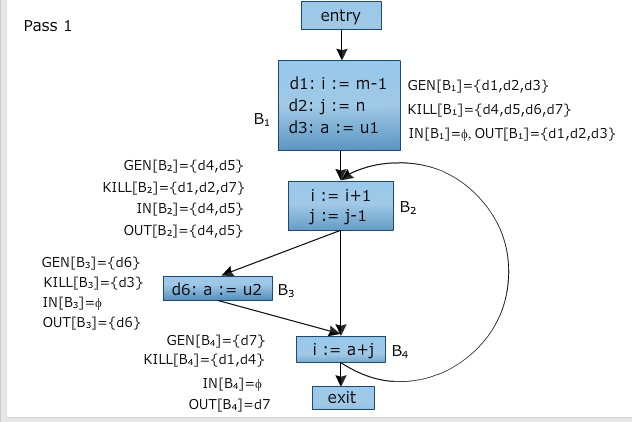
\includegraphics[width=\linewidth]{rdex1.jpg}
      \caption{Pass 1}\label{fig:awesome_image1}
    \endminipage\hfill
    \minipage{0.32\textwidth}
      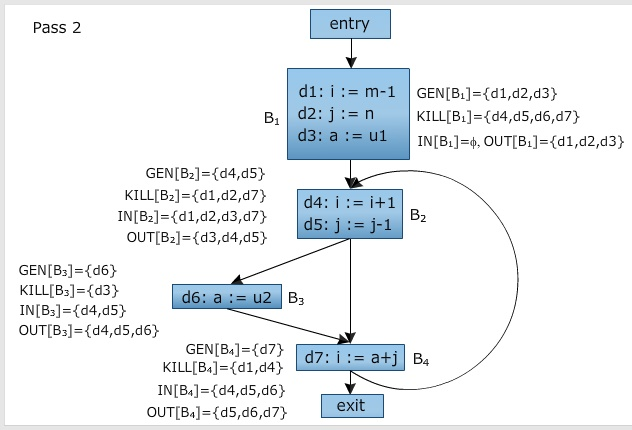
\includegraphics[width=\linewidth]{rdex2.jpg}
      \caption{Pass 2}\label{fig:awesome_image2}
    \endminipage\hfill
    \minipage{0.32\textwidth}%
      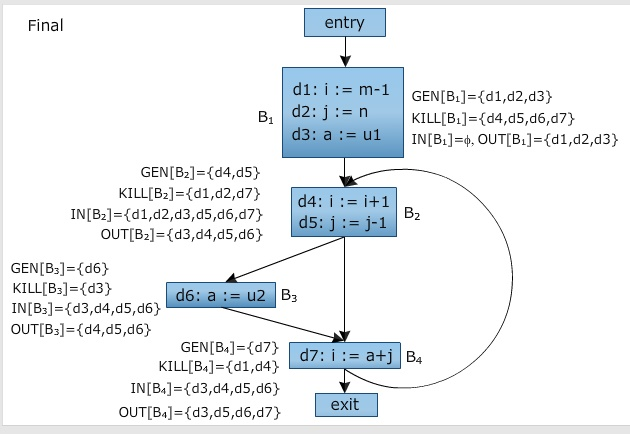
\includegraphics[width=\linewidth]{rdex3.jpg}
      \caption{Pass 3}\label{fig:awesome_image3}
    \endminipage
\end{figure}



\subsection{ Live    Variable    Analysis   }

In compilers, live variable analysis (or simply liveness analysis)
 is a classic data-flow analysis to calculate the variables that 
 are live at each point in the program. A variable is live at 
 some point if it holds a value that may be needed in the future, 
 or equivalently if its value may be read before the next time 
 the variable is written to. \footnote{based on Wikipedia}

\subsubsection{Motivation}


For dead code elimination.
\subsection{}


\section{ Live Variabl Analysis   }

In compilers, live variable analysis (or simply liveness analysis)
is a classic data-flow analysis to calculate the variables that
are live at each point in the program. A variable is live at
some point if it holds a value that may be needed in the future,
or equivalently if its value may be read before the next time
the variable is written to. \footnote{based on Wikipedia}

\subsection{Motivation}

Programs may contain

\begin{itemize}
	\item code which gets executed but which has no useful
	      effect on the program's overall result;
	\item occurrences of variables being used before they
	      are defined;\footnote{we can use liveness information to find undefined variables.}
	\item many variables which need to be allocated
	      registers and/or memory locations for compilation.\footnote{Two	variables	can	use	the	same	register	if	they	are	never	in	use	at	the
		      same time(i.e,	never	simultaneously live). Register	allocation
		      uses liveness information.}

\end{itemize}

The concept of variable liveness is useful in dealing
with all three of these situations.


Liveness analysis is highly used for \textbf{register allocation}(If variable \texttt{x} is live in a basic block b, it is a potential candidate for
register allocation) and \textbf{dead code elimination}(If variable \texttt{x} is not live after an assignment \texttt{x =...}, then the assignment is
redundant and can be deleted as dead code).


\subsection{Problem formulation}
Liveness is a data-flow property of variables:
“Is the value of this variable needed?” We therefore
usually consider liveness from an instruction's
perspective: each instruction (or node of the
flowgraph) has an associated set of live variables.


\subsection{Semantic vs. syntactic}


There are two kinds of variable liveness : Semantic liveness and Syntactic liveness.


A variable x is \textbf{semantically} live at a node n if there is
some execution sequence starting at n whose (externally
observable) behaviour can be affected by changing the
value of x. Semantic liveness is concerned with
the execution behaviour of the program.

A variable is \textbf{syntactically} live at a node if there is a
path to the exit of the flow graph along which its
value may be used before it is redefined. Syntactic liveness is concerned with properties of
the syntactic structure of the program.


So what is the difference between Semantic liveness and Syntactic liveness? syntactic liveness
is a computable approximation of semantic liveness.


Consider the example \ref{lst:expr2}


\begin{lstlisting}[language=C,frame=single, caption=An example to illustrate semantic syntatic,label = lst:expr2]
    int t = x * y;
    if ((x+1)*(x+1) == y) {
     t = 1;
    }
    if (x*x + 2*x + 1 != y) {
     t = 2;
    }
    return t;
\end{lstlisting}

In fact, t is dead in node \texttt{int t = x * y;} because one of the conditions will be true,
so on every execution path t is redefined before it is returned.
The value assigned by the first instruction is never used.


But on read path from Figure \ref{fig:liveex} through the
flowgraph, t is not
redefined before it's used,
so t is syntactically live at
the first instruction.Note that this path never
actually occurs during
execution.

\begin{figure}[h]
	\centering
	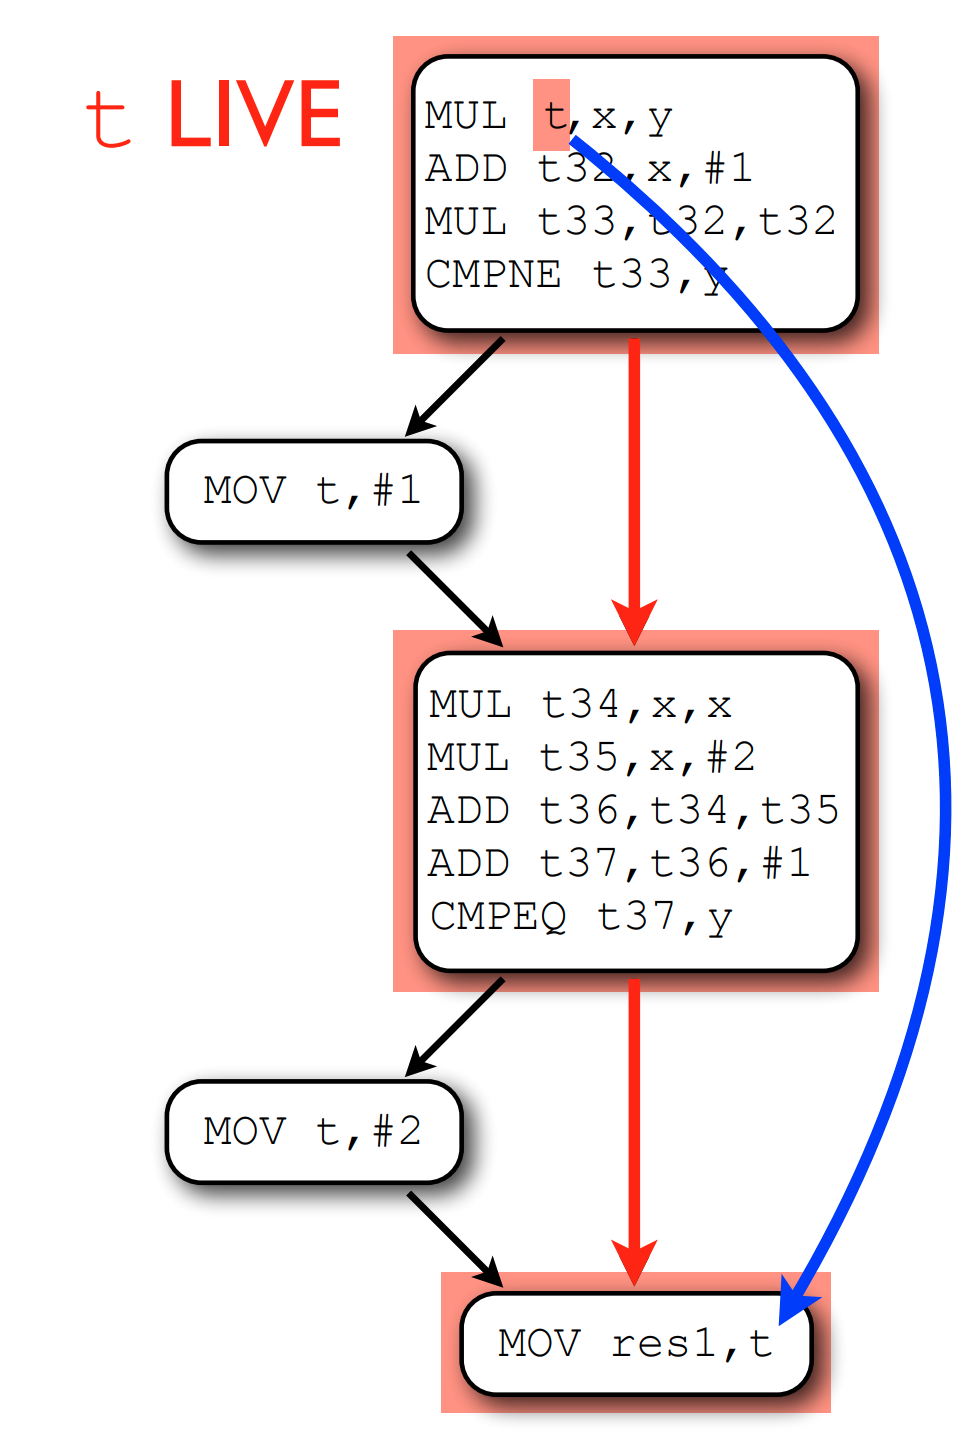
\includegraphics[width=0.3\textwidth]{liveex.png}
	\caption{CFG for \ref{lst:expr2}}
	\label{fig:liveex}
\end{figure}


\subsection{Summary}


\begin{center}
	\begin{tabular}{|c|c|}
		\hline Direction                         & Backward                                            \\
		\hline Domain                            & Sets	of	variables                                     \\
		\hline Meet operator                     & \( \cup \)                                          \\
		\hline Top(T)                            & $\phi$                                              \\
		\hline Bottom                            & Universal Set                                       \\
		\hline Boundary condition                & $\mathrm{IN[EXIT]} = \phi$                          \\
		\hline Initialization for internal nodes & $\mathrm{IN[B]} = \phi$                             \\
		\hline Finited escending chain?          & \checkmark                                          \\
		\hline Transfer function                 & $f_b(x) = \mathrm{USE}_b \cup (x - \mathrm{DEF}_b)$ \\
		\hline Monotone\&Distributive?           & \checkmark                                          \\
		\hline
	\end{tabular}
\end{center}




\subsection{Strongly Live Variables Analysis\cite{LiveVari29:online}}

A variable is strongly live if
\begin{itemize}

	\item it is used in a statement other than assignment statement, or
	      (same as simple liveness)
	\item it is used in an assignment statement defining a variable that is
	      strongly live
\end{itemize}


\begin{figure}[H]
	\centering
	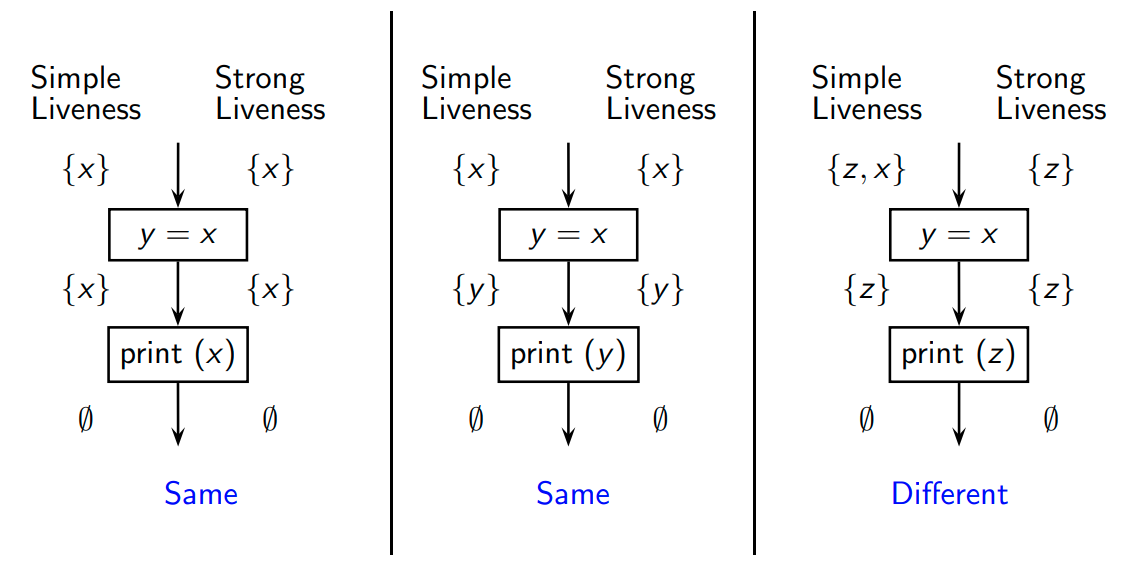
\includegraphics[width=0.7\textwidth]{p217.png}
	\caption{Understanding Strong Liveness}
	\label{fig:p217}
\end{figure}


A variable is live at a program
point if its current value is likely
to be used later. We want to compute the smallest
set of variables that are live. Simple liveness considers every
use of a variable as useful. Strong liveness checks the liveness
of the result before declaring the
operands to be live. Strong liveness is more precise
than simple liveness. The transfer function of Strongly Live Variables Analysis is shwon
below:


$$
	f_n(X)= \begin{cases}(X-\{y\}) \cup(Opd(e) \cap \mathbb{V}ar) & n \text { is } y=e, e \in \mathbb{E}pr, y \in X \\ X-\{y\} & n \text { is input }(y) \\ X \cup\{y\} & n \text { is use }(y) \\ X & \text { otherwise }\end{cases}
$$


The first case means that If \texttt{y} is not strongly live, the
assignment is skipped using
the “otherwise” clause

\begin{figure}[H]
	\centering
	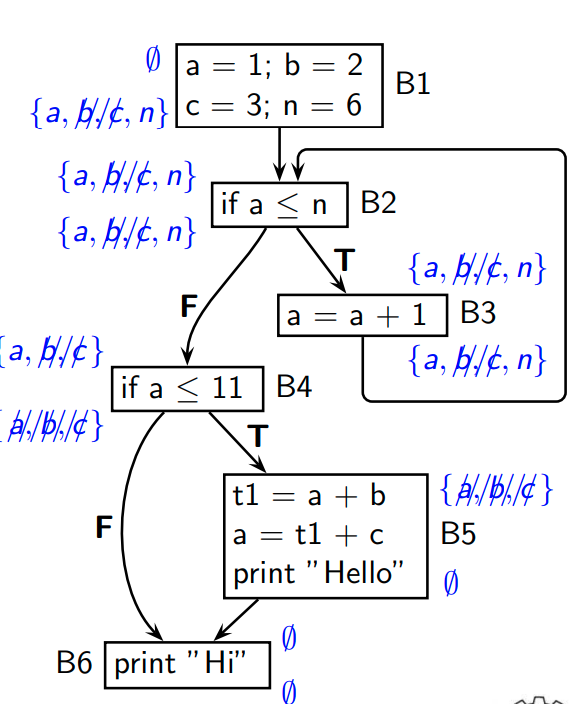
\includegraphics[width=0.4\textwidth]{p218.png}
	\caption{Simple Liveness VS. Strong Liveness.}
	\label{fig:p218}
\end{figure}

\section{Reaching Definitions}

The Reaching Definitions Problem is a data-flow problem used to answer the
following questions: Which definitions of a variable \textit{X} reach a given use of \textit{X} in
an expression? Is \textit{X} used anywhere before it is defined? A definition\textit{d} reaches a point \textit{p} if there exists path 
from the point immediately following \textit{d} to \textit{p} such that \textit{d} is not killed(overwritten) along that path.



\subsection{Iterative   Algorithm}

Here is the iterative  algorithm.



\begin{algorithm}
    \caption{Reaching Defintions:Iterative Algorithm}\label{alg:reachingdefiterative}
    \hspace*{\algorithmicindent} \textbf{Input: control flow graph CFG = (N, E, Entry, Exit) } \\
   
    
    \begin{algorithmic}
   
    \State out[Entry] = $\emptyset$ \algorithmiccomment{Boundary condition}

    \For{\texttt{each basic block B other than Entry}}
        \State \texttt{out[B] = $\emptyset$} \algorithmiccomment{Initialization for iterative algorithm }
    \EndFor
    \While{Changes to any out[] occur}
        \For{\texttt{each basic block B other than Entry}}
        \State \texttt{$in[B] =  \cup (out[p])$, for all predecessors p of B}
        \State \texttt{$out[B] = f_B(in[B])$} \algorithmiccomment{$out[B]=gen[B]\cup (in[B]-kill[B]) $ }
        \EndFor

    \EndWhile
    \end{algorithmic}
\end{algorithm}




\subsection{ Worklist   Algorithm}

\begin{algorithm}
    \caption{Reaching Defintions:Worklist Algorithm}\label{alg:reachingdefiterative}
    \hspace*{\algorithmicindent} \textbf{Input: control flow graph CFG = (N, E, Entry, Exit) } \\
   
    
    \begin{algorithmic}
   
    \State out[Entry] = $\emptyset$ \algorithmiccomment{Boundary condition}
    \State \textcolor{blue}{ChangedNodes = N}   
    \For{\texttt{each basic block B other than Entry}}
        \State \texttt{out[B] = $\emptyset$} \algorithmiccomment{Initialization for iterative algorithm }
    \EndFor
    \While{ChangedNodes $\neq \emptyset$}
        \State \textcolor{blue}{Remove i from ChangedNodes}
        \State $in[B] =  \cup (out[p])$, for all predecessors p of B
        \State \textcolor{blue}{$oldout = out[i]$}
        \State $out[i] = f_i(in[i])$ \algorithmiccomment{$out[i]=gen[i]\cup (in[i]-kill[i]) $ }
        \If {\textcolor{blue}{oldout} $\neq out[i]$}

            \For{\texttt{all \textcolor{blue}{successors s of i}}}
                \State \textcolor{blue}{add s to ChangedNodes}
            \EndFor
        \EndIf

    \EndWhile
    \end{algorithmic}
\end{algorithm}



\subsection{Example}
Here comes an example of reaching definition.

\begin{figure}[!htb]
    \minipage{0.32\textwidth}
      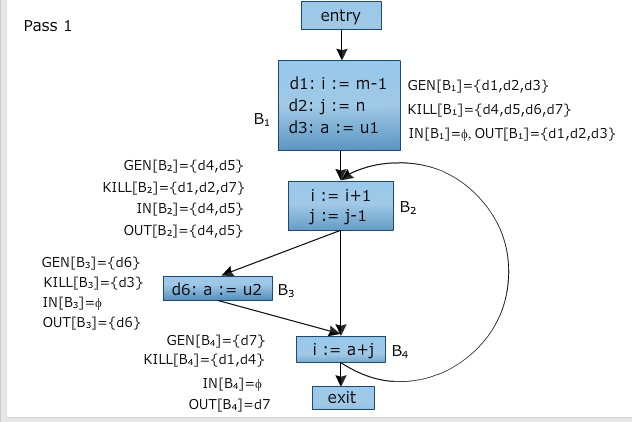
\includegraphics[width=\linewidth]{rdex1.jpg}
      \caption{Pass 1}\label{fig:awesome_image1}
    \endminipage\hfill
    \minipage{0.32\textwidth}
      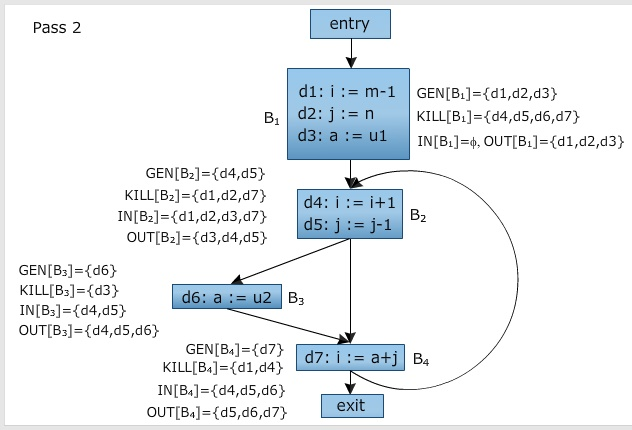
\includegraphics[width=\linewidth]{rdex2.jpg}
      \caption{Pass 2}\label{fig:awesome_image2}
    \endminipage\hfill
    \minipage{0.32\textwidth}%
      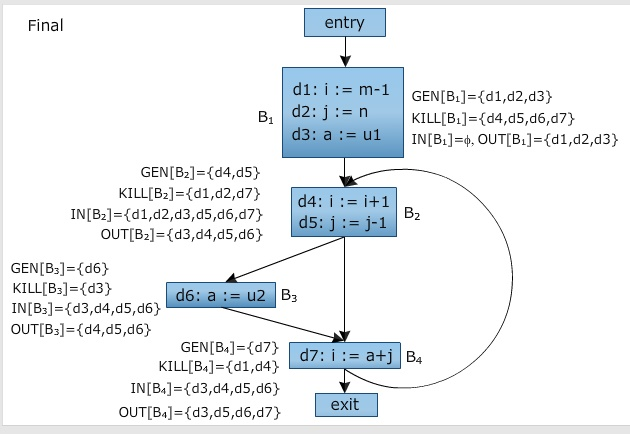
\includegraphics[width=\linewidth]{rdex3.jpg}
      \caption{Pass 3}\label{fig:awesome_image3}
    \endminipage
\end{figure}
\newpage

\section{Available Expressions Analysis}

\subsection{Motivation}

Programs may contain code whose result is needed, but in which some computation is simply a redundant
repetition of earlier computation within the same program. The concept of expression availability is useful in dealing with this situation.


\subsection{Backgroud Knowledge}

Any given program contains a finite number of expressions (i.e. computations which potentially
produce values),so we may talk about the set of all expressions of a program. Consider the program in
\ref{lst:expression1}




\begin{lstlisting}[language=C,frame=single, caption=An simple example containing some expressions ,label = lst:expression1]
    int z = x * y; 
    print s + t; 
    int w = u / v;
\end{lstlisting}


This program contian expression \texttt{x*y,s+t,u/v}.



\subsection{Problem Formulation}


Availability is a data-flow property of expressions: “Has the value of this expression already been computed?”
At each instruction, each expression in the programis either available or unavailable. So each instruction(or node of the flowgraph) has
an associated set of available expression.



\subsection{Semantic vs. Syntactic}

An expression is \textit{semantically} available at a node n if its value gets computed
(and not subsequently invalidated) along every execution sequence ending at n.

\begin{figure}[!htb]
	\minipage{0.5\textwidth}
	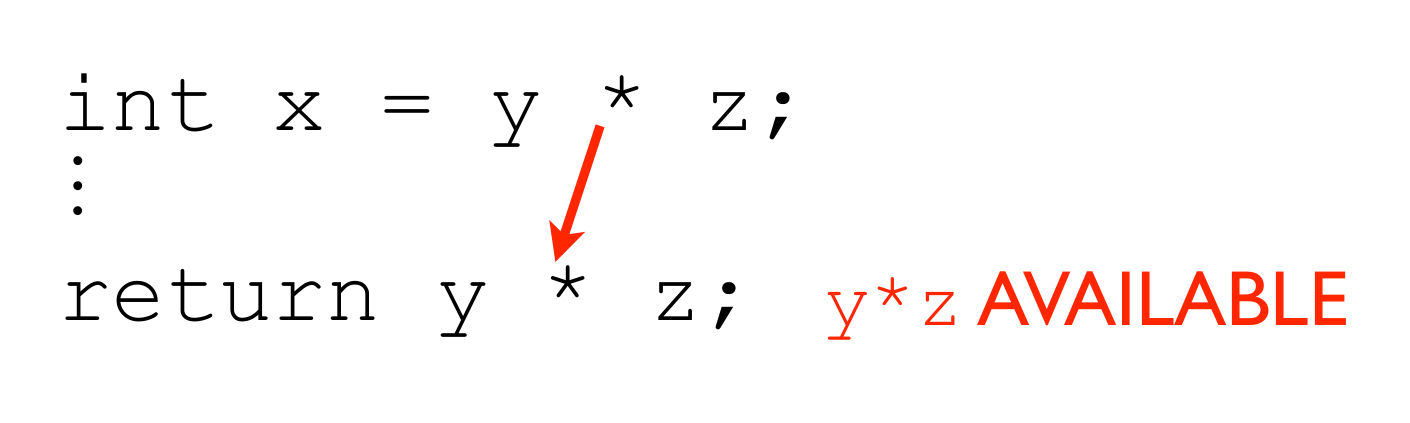
\includegraphics[width=\linewidth]{p1.png}
	\caption{Available expression example}\label{fig:p1}
	\endminipage\hfill
	\minipage{0.5\textwidth}
	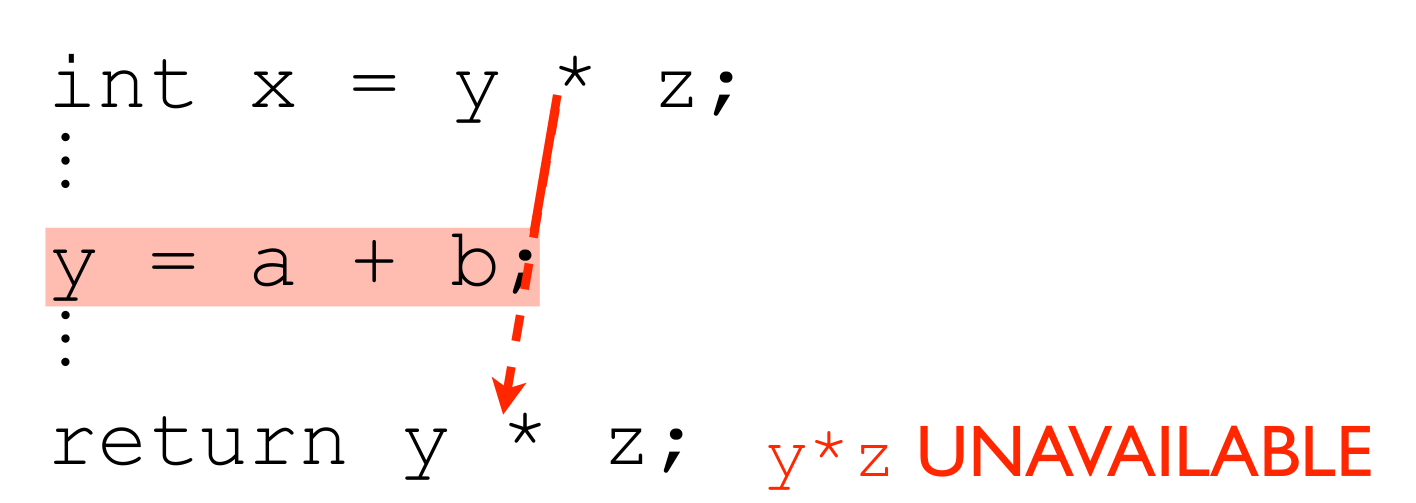
\includegraphics[width=\linewidth]{p2.png}
	\caption{unavailable expression example}\label{fig:p2}
	\endminipage
\end{figure}


An expression is \textit{syntactically} available at a node n if its value gets computed
(and not subsequently invalidated) along every path from the entry of the flowgraph to n.


\begin{figure}[!htb]
	\minipage{0.5\textwidth}
	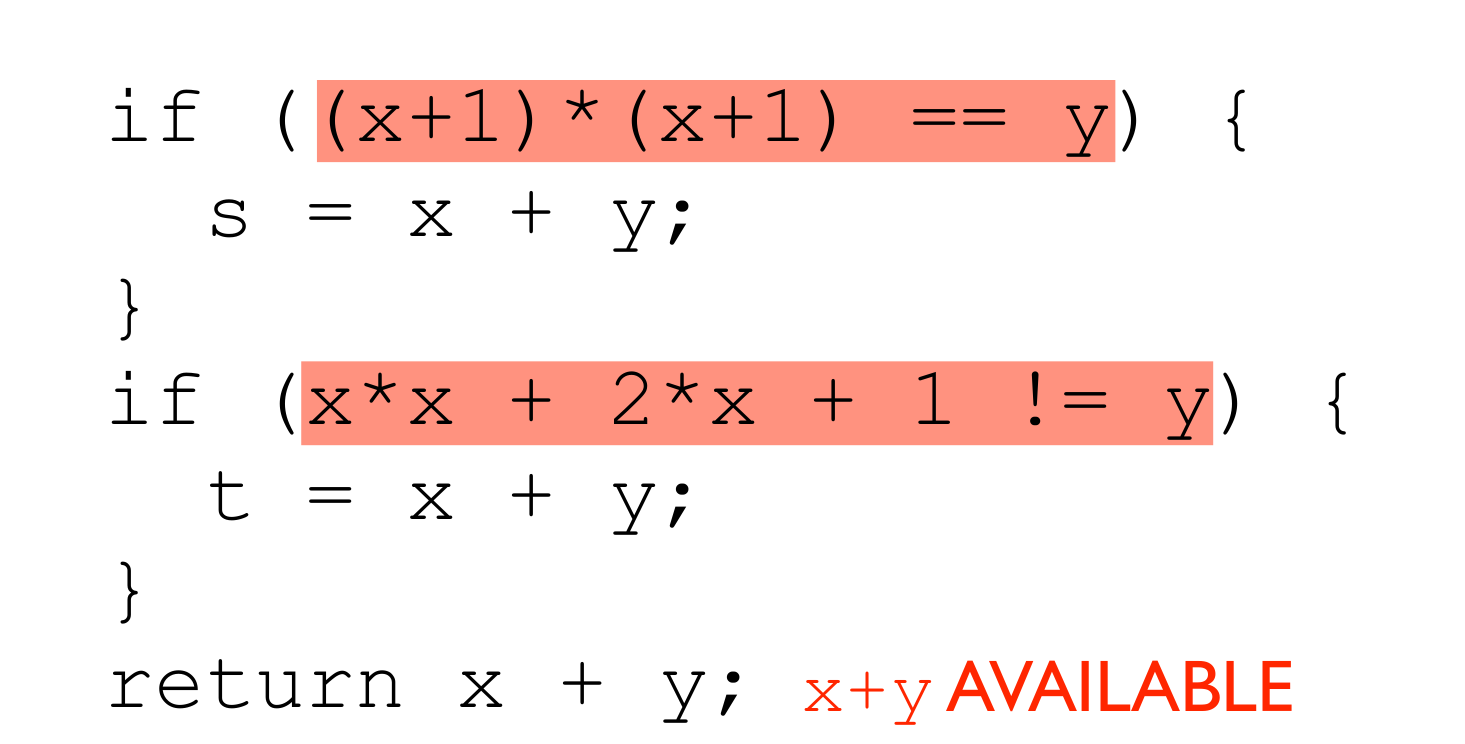
\includegraphics[width=\linewidth]{p4.png}
	\caption{x+y is semantically available}\label{fig:p4}
	\endminipage\hfill
	\minipage{0.4\textwidth}
	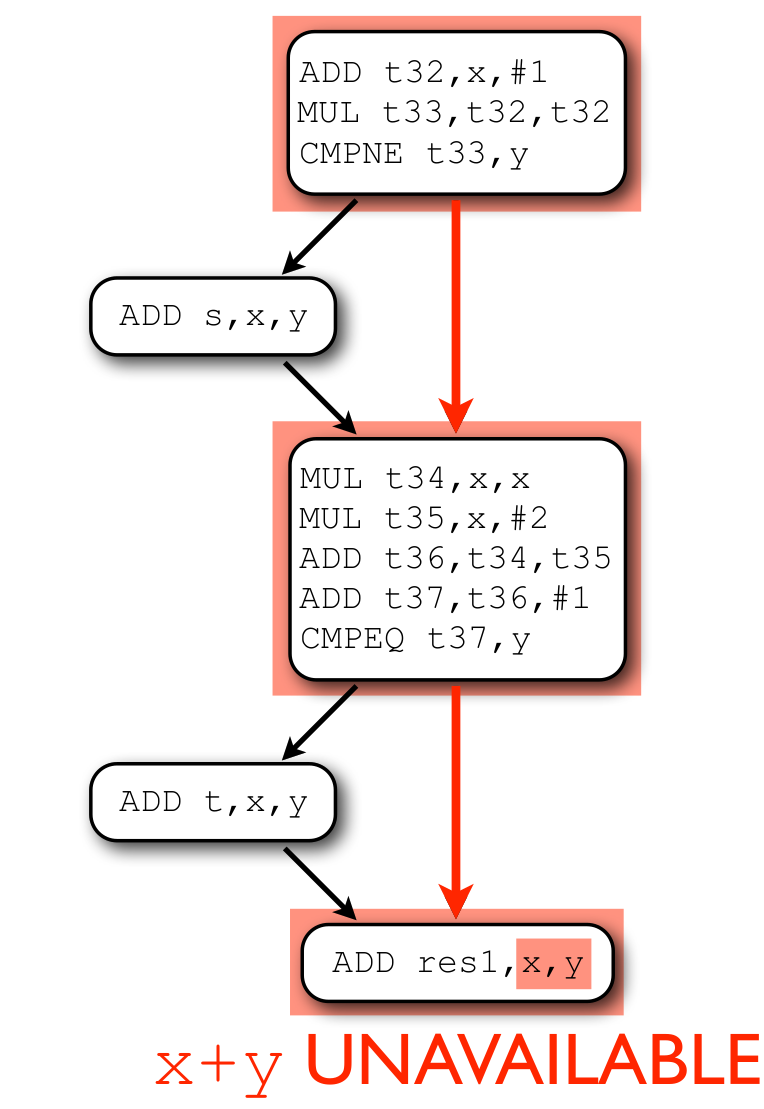
\includegraphics[width=\linewidth]{p3.png}
	\caption{x+y is syntactically unavailable}\label{fig:p3}
	\endminipage
\end{figure}


On the path in red from Figure \ref{fig:p3} through the flowgraph, \(x+y\) is only
computed once, so \(x+y\) is syntactically unavailable at the last instruction.


Whereas with live variable analysis we found safety in assuming that
more variables were live, here we find safety in assuming that fewer
expressions are available. Because if an expression is deemed to be available, we
may do something dangerous (e.g. remove an instruction which recomputes its value).
So sometimes safe means more, but sometimes means less.

\begin{figure}[H]
	\minipage{0.5\textwidth}
	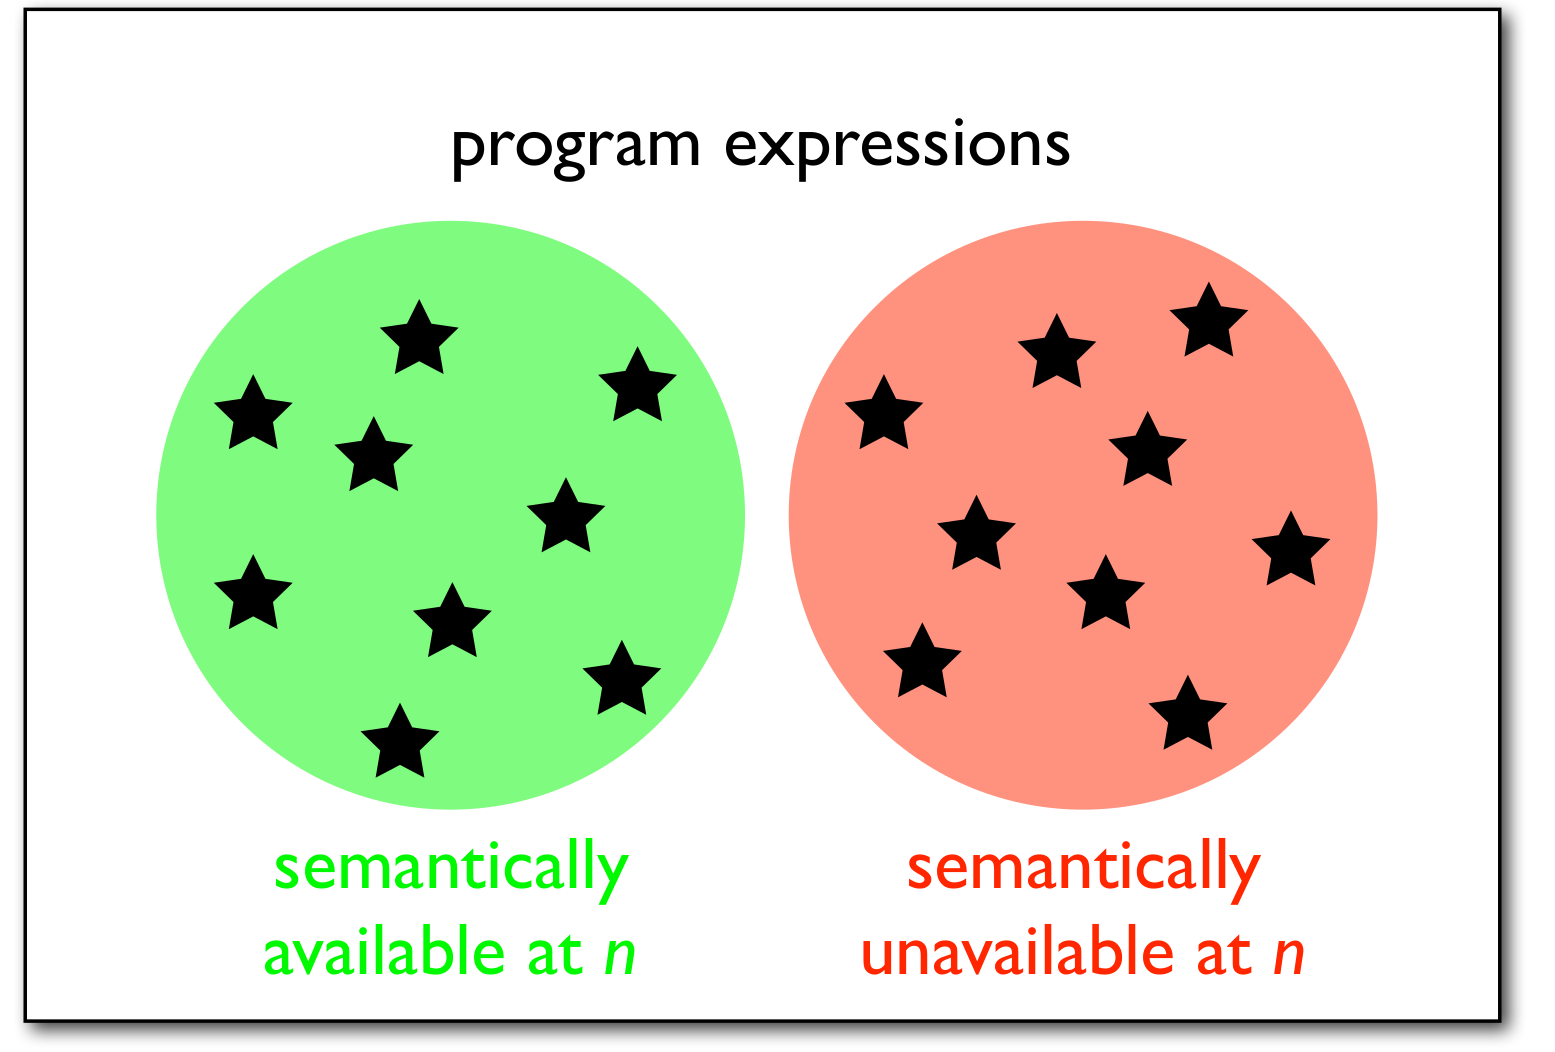
\includegraphics[width=\linewidth]{p5.png}
	\caption{Semantic vs. syntactic}\label{fig:p5}
	\endminipage\hfill
	\minipage{0.5\textwidth}
	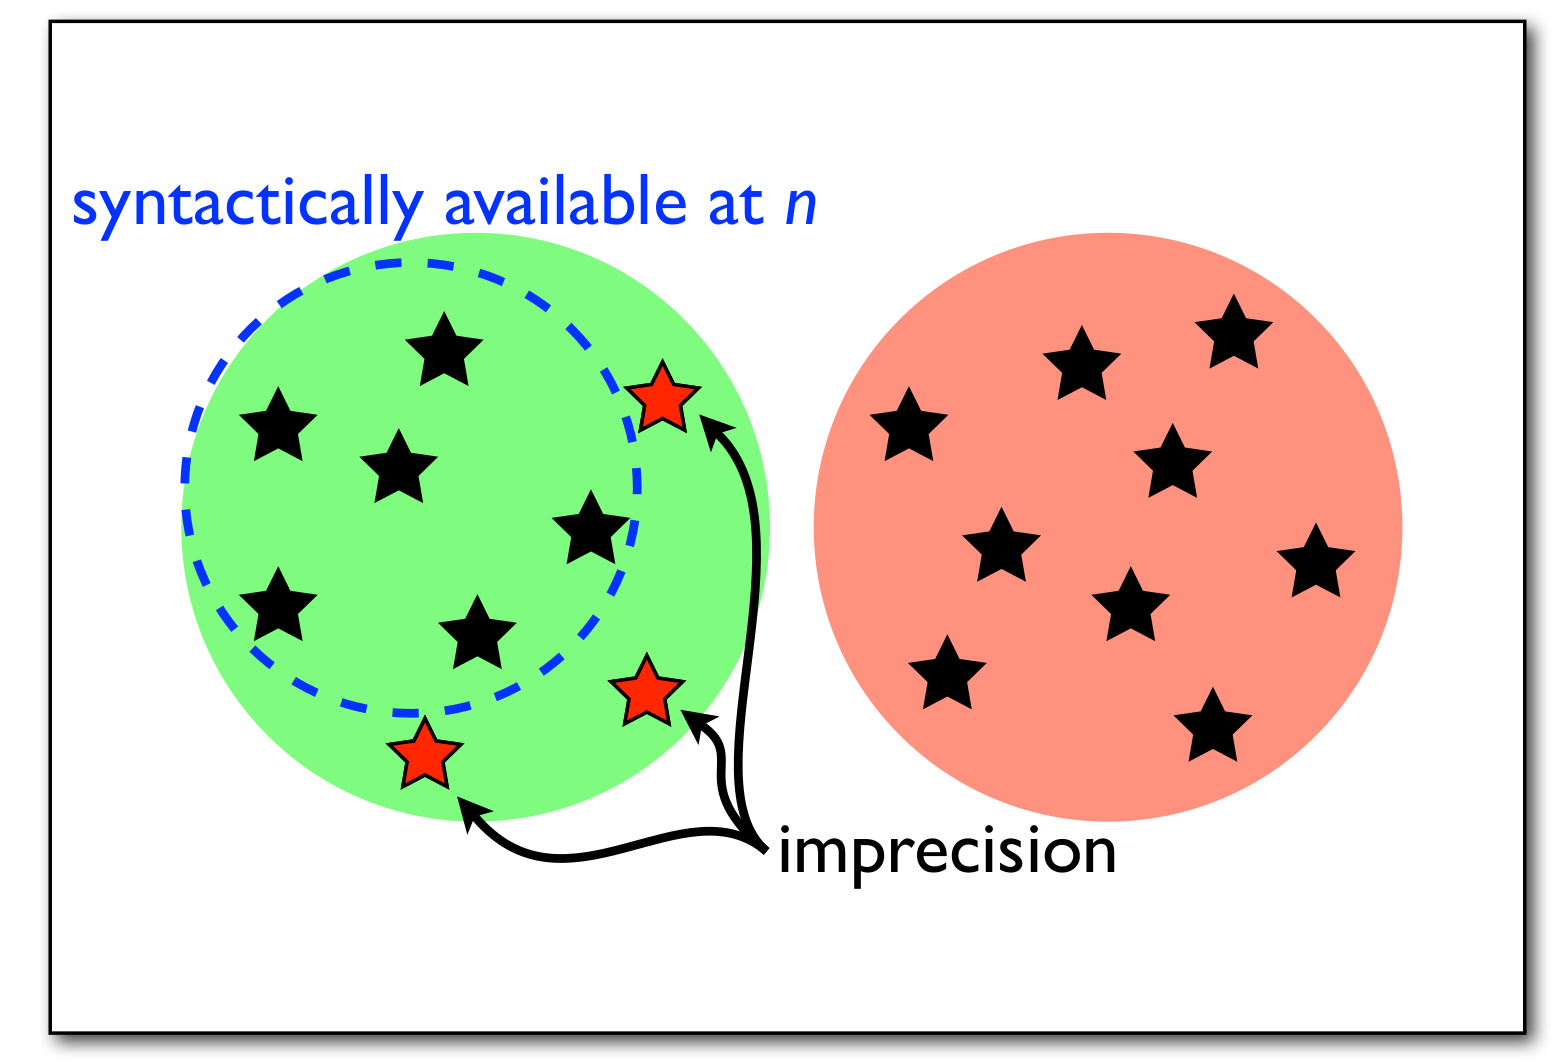
\includegraphics[width=\linewidth]{p6.png}
	\caption{Semantic vs. syntactic}\label{fig:p6}
	\endminipage
\end{figure}


\subsection{Summary}


\begin{center}
	\begin{tabular}{|c|c|}
		\hline Direction                         & Forward                                           \\
		\hline Domain                            & Sets of expressions                                    \\
		\hline Meet operator                     & \( \cap \)                                          \\
		\hline Top(T)                            & Universal Set                                             \\
		\hline Bottom                            & $\phi$                                     \\
		\hline Boundary condition                & $\mathrm{OUT[ENTRY]} = \phi$                          \\
		\hline Initialization for internal nodes & $\mathrm{OUT[B]} = T$                             \\
		\hline Finited escending chain?          & \checkmark                                          \\
		\hline Transfer function                 & $f_b(x) = \mathrm{Gen}_b \cup (x - \mathrm{Kill}_b)$ \\
		\hline Monotone\&Distributive?           & \checkmark                                          \\
		\hline $\mathrm{Kill}_b$ & all E such that block b defines a variable in E \\
    \hline $\mathrm{Gen}_b$ & all E such that block b evaluates E and doesn’t later kill it \\
    \hline
	\end{tabular}
\end{center}
\section{Foundations of Data Flow Analysis}



Having shown several useful examples of the data-flow abstraction, 
we now study the family of data-flow schemas as a whole, abstractly. 
We shall answer several basic questions about data-flow algorithms formally:

\begin{itemize}

\item Under what circumstances is the iterative algorithm used in data-flow analysis correct?
\item How precise is the solution obtained by the iterative algorithm?
\item Will the iterative algorithm converge?
\item How fast is the convergence?
\end{itemize}


\subsection{Partial Order}\footnote{Based on \url{https://pages.cs.wisc.edu/~horwitz/CS704-NOTES/2.DATAFLOW.html}}

A binary relation R on a set S is called a partial ordering(poset), or partial order if and only if it is:

\begin{itemize}
\item \textbf{Reflexive} \(x \leq x\)
\item \textbf{Antisymmetric} if \(x \leq y\) and \(y \leq x\) then \(x = y\)
\item \textbf{Transitive} if \(x \leq y\) and \(y \leq z\) then \(x \leq z\)
\end{itemize} 



\subsection{Lattices}

A lattice is a poset in which every pair of elements has:

\begin{itemize}
\item a Least Upper Bound (the join of the two elements), and
\item a Greatest Lower Bound (the meet of the two elements).
\end{itemize}    



\subsection{Complete lattices}


A complete lattice is a lattice in which all subsets have a greatest lower bound 
and a least upper bound (the bounds must be in the lattice, but not necessarily 
in the subsets themselves). Note that Every finite lattice (i.e., S is finite) is complete.


\subsection{Monotonic and distributive functions}

A function f: L → L (where L is a lattice) is monotonic iff for all x,y in L: x ⊆ y implies f(x) ⊆ f(y).

A function f: L → L (where L is a lattice) is distributive iff for all x,y in L: f(x meet y) = f(x) meet f(y).

Every distributive function is also monotonic (proving that could be good practice!) but not vice versa. For the GEN/KILL dataflow problems, all dataflow functions are distributive. For constant propagation, all functions are monotonic, but not all functions are distributive.


\subsection{Fixed points}

x is a fixed point of function f iff f(x) = x.

\subsection{Meet Operator}



\section{LLVM}




\subsubsection{PGO and LLVM}

Profile Guided Optimizations.

\subsection{Profile Guided Transforms}

\subsubsection{Spill Placement}
registers

\subsubsection{Code Layout}

Code layout \cite{raman2022learning} is the process of ordering the blocks of the CFG. This order dictates the
placement of instructions within those blocks in memory. By inserting branch instructions at the end of the basic blocks,
the compiler can layout the blocks in any order.  Consider the
Control Flow Graph (CFG) in Figure \ref{fig:p7}. Figures \ref{fig:p8} and \ref{fig:p9}
show two possible layouts of the CFG. In both theese layouts,
a block is followed by one of its successor blocks that is
not yet laid out. Consider block A, for example. It has two
successors in the CFG. Only one of the successors B or C 
can be placed immediately following A and is known as the
\textbf{fall-through block}. In Figure \ref{fig:p8}, B is the fall-through block
and in the layout in Figure \ref{fig:p9}, C is the fall-through block.
The choice of which block to place as the fall-through block
has performance implications. If control is often transferred
to C from A often during program execution, then placing
C next to A has the following advantages:


\begin{figure}[!htb]
    \minipage{0.5\textwidth}
      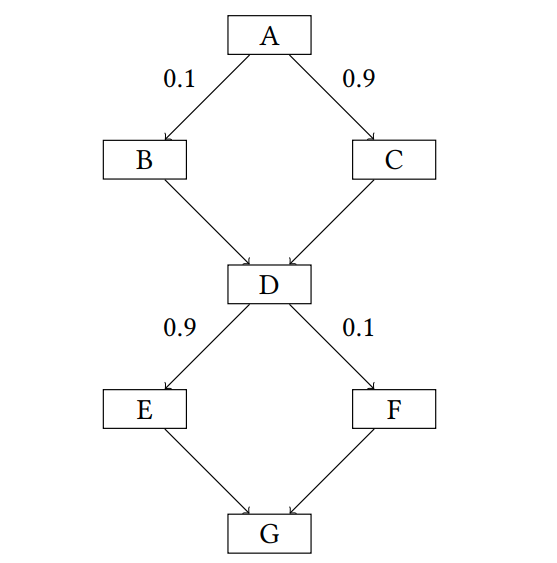
\includegraphics[width=\linewidth]{p7.png}
      \caption{CFG}\label{fig:p7}
    \endminipage\hfill
    \minipage{0.25\textwidth}
      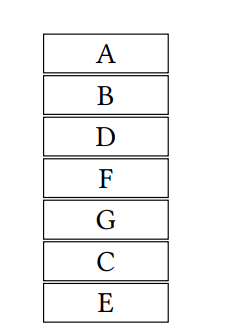
\includegraphics[width=\linewidth]{p8.png}
      \caption{Layout 1}\label{fig:p8}
    \endminipage\hfill
    \minipage{0.25\textwidth}
      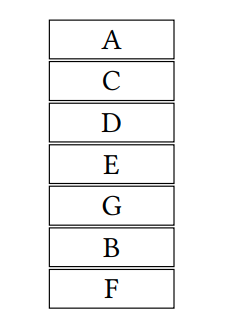
\includegraphics[width=\linewidth]{p9.png}
      \caption{Layout 2}\label{fig:p9}
    \endminipage\hfill
    \caption{Code Layout}
\end{figure}




\begin{itemize}
\item Since the branch at the end of A is mostly not-taken,
the frontend of the processor's pipeline is less likely to
be stalled if it is an out-of-order superscalar processor.
\item As the cacheline containing the last instruction of A
also contains instructions that are more likely to execute (from block C), instruction cache utilization is
likely to be better.
\end{itemize}

In the LLVM compiler, the \texttt{MachineBlockPlacement} pass
performs code layout optimization. This pass relies on the
branch probability analysis which provides, for each branch
instruction, the probability of the branch being taken.
\texttt{MachineBlockPlacement} is just one of the many transformation passes that make use of branch probability analysis.
Branch probability analysis is used in another analysis called
block frequency analysis that provides relative frequencies of
basic blocks within a function. Block frequency analysis is
used by optimizations such as inlining, spill-code placement 
in register allocation among others.

\subsubsection{Hot/Cold Partitioning}

\begin{figure}[!htb]
    \minipage{0.33\textwidth}
      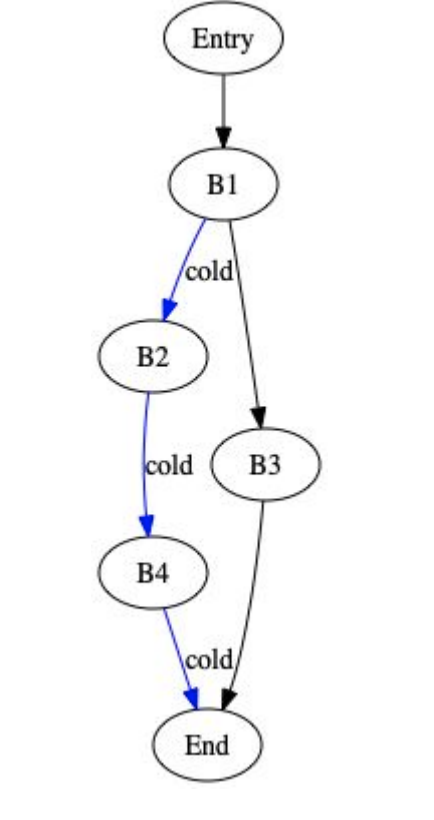
\includegraphics[width=\linewidth]{p10.png}
      \caption{CFG}\label{fig:p10}
    \endminipage\hfill
    \minipage{0.33\textwidth}
      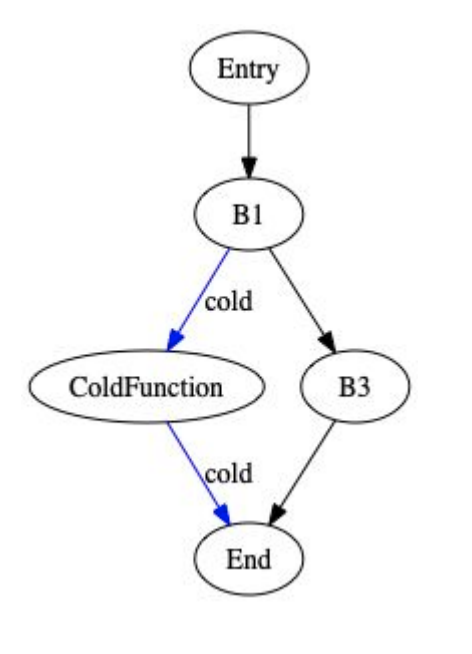
\includegraphics[width=\linewidth]{p11.png}
      \caption{Layout 1}\label{fig:p11}
    \endminipage\hfill
    \minipage{0.33\textwidth}
      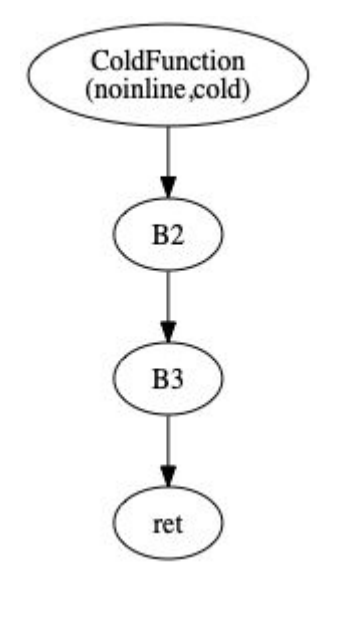
\includegraphics[width=\linewidth]{p12.png}
      \caption{Layout 2}\label{fig:p12}
    \endminipage\hfill
    \caption{Code Layout}
\end{figure}


Hot Cold splitting is an optimization to improve instruction locality. It is used to outline basic blocks which execute less frequently. The hot/cold splitting pass identifies cold basic blocks and moves them into separate functions. The linker can then put newly-created cold functions away from the rest of the program . The idea here is to have these cold pages faulted in relatively infrequently, and to improve the memory locality of code outside of the cold area.

The algorithm is novel in the sense it is based on region and implemented at the IR level. Because it is implemented at the IR level, all the backend targets benefit from this implementation. Other implementations of hot-cold splitting outline each basic block separately and are implemented at the RTL level.


What applications will benefit from Hot/Cold Spliting?

\begin{itemize}

\item High cache misses(A giant app on a small device)
\item High start-up time

\end{itemize}


\subsubsection{Inliner}



\subsubsection{Outlining \& Merging}

With PGO information, we can do more aggressive outlining of cold regions in the inline candidate function. This contrasts with the scheme of keeping only the 'early return' portion of the inline candidate and outlining the rest of the function as a single function call.

Support for outlining multiple regions of each function is added, as well as some basic heuristics to determine which regions are good to outline. Outline candidates limited to regions that are single-entry \& single-exit. Also we don't account for live-ranges we may be killing across the region with a function. These are enhancements we can consider in another patch.

Fallback to the regular partial inlining scheme is retained when either i) no regions are identified for outlining in the function, or ii) the outlined function could not be inlined in any of its callers.




\printbibliography

\end{document}
